%    JJJ    AA     CCCCCC KKK   K TTTTTT HH  HH EEEEEE BBBBBB UU  UU SSSSSS    CCCCCC OOOOOO MM  MM
%    JJJ   AAAA    CCCCCC KKK  K  TTTTTT HH  HH EEEEEE BB   B UU  UU SSS       CCCCCC OOOOOO MM  MM
%    JJJ  AA  AA   CC     KKK K     TT   HHHHHH EEE    BB   B UU  UU SSS       CC     OO  OO MMMMMM
%    JJJ AA    AA  CC     KKKK      TT   HHHHHH EEEEEE BBBBBB UU  UU  SSSSS    CC     OO  OO M MM M
%    JJJ AAAAAAAA  CC     KKK K     TT   HH  HH EEE    BB   B UU  UU    SSS    CC     OO  OO M MM M
% JJJJJJ AA    AA  CCCCCC KKK  K    TT   HH  HH EEEEEE BB   B UUUUUU    SSS .. CCCCCC OOOOOO M MM M
% JJJJJJ AA    AA  CCCCCC KKK   K   TT   HH  HH EEEEEE BBBBBB UUUUUU SSSSSS .. CCCCCC OOOOOO M MM M
% 
% Texte Geschrieben von Stefan Bopp und Chantal Frunz
% Mehr Informationen sind auf jackthebus.com zu finden
%
%\begin{wrapfigure}{R}{0.45\textwidth} 
%  \begin{centering}
%    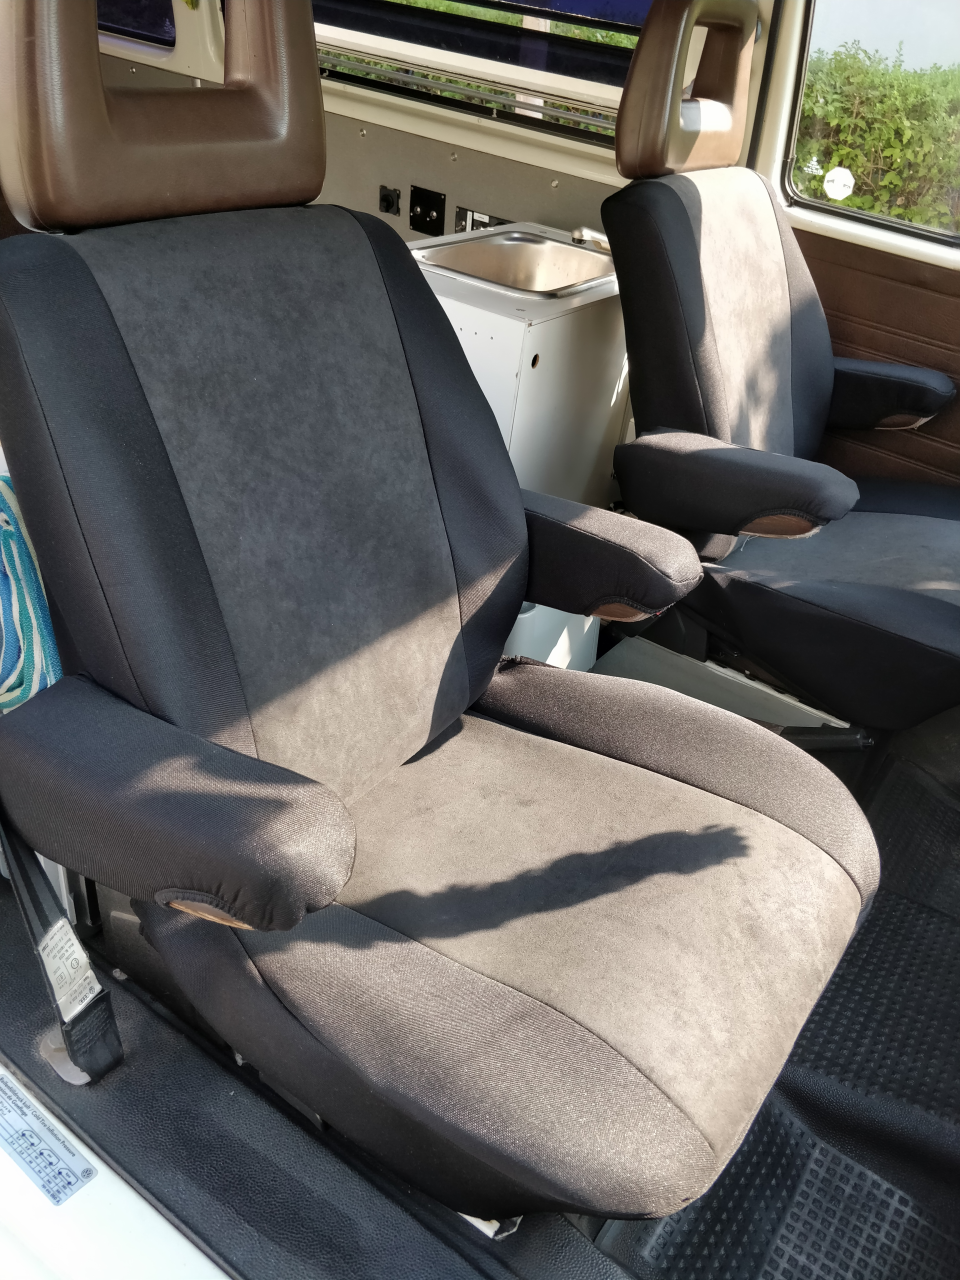
\includegraphics[width=0.4\textwidth, height=5cm, keepaspectratio]{../Bilder/Sylt/1.jpg}
%    \caption{Regen}
%  \end{centering}
%\end{wrapfigure} 

%\begin{figure}[b]
%   \centering
%      %\subfloat[CAPTION]{BILDERCODE}\qquad
%   \subfloat{\includegraphics [width=0.3\textwidth]{../Bilder/Sylt/2.jpg}}\quad
%   \subfloat{\includegraphics [width=0.3\textwidth]{../Bilder/Sylt/3.jpg}}\quad
%   \subfloat{\includegraphics [width=0.3\textwidth]{../Bilder/Sylt/4.jpg}}\quad
%   \caption[Meran]{Meran}
%\end{figure}

%\begin{figure}[hb]
%    \centering
%    \includegraphics[width=\textwidth]{../Bilder/Sylt/7.jpg}
%    \caption{Da sind sie ja...}
%    \label{img:Sardinien}
%\end{figure}

\subsection{Einleitung} 

\begin{wrapfigure}{R}{0.35\textwidth} 
  \begin{centering}
    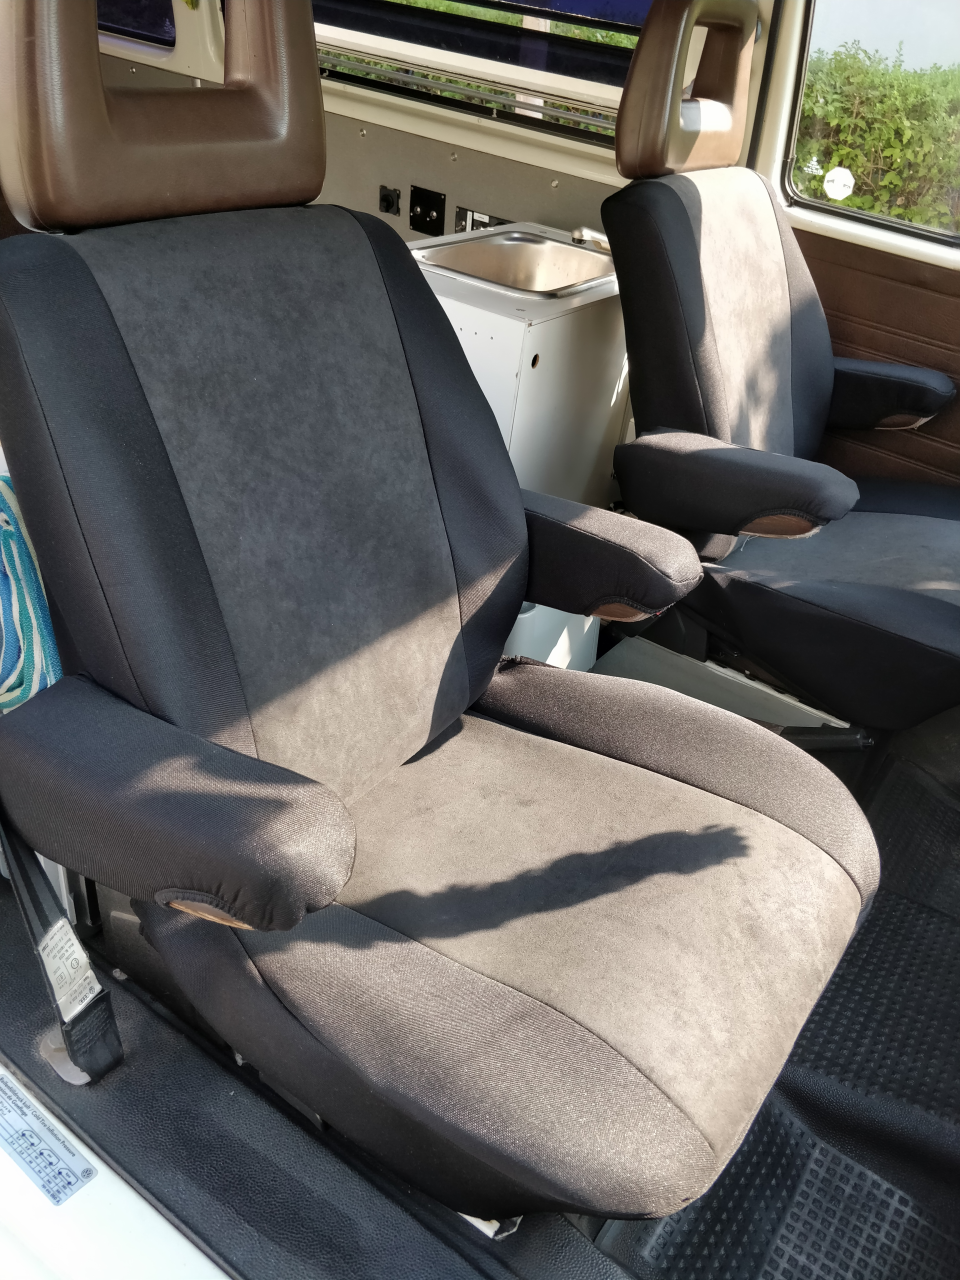
\includegraphics[width=0.4\textwidth, height=5cm, keepaspectratio]{../Bilder/Sylt/1.jpg}
    \caption{Neue Sitzbezüge}
  \end{centering}
\end{wrapfigure} 

Ein Geburtstag und eine damit verbundene Einladung lockte uns für einmal in den Norden.
Die Hitzewelle welche die Schweiz und Europa fest im Griff hatte liess uns von tieferen Temperaturen träumen.hu
Eine zweiwöchige Geschäftsreise nach Phoenix mit Spitzentemperaturen von 47°C erhöhten den Wunsch nach angenehmere Temperaturen nur noch mehr.
Das Ziel sollte Sylt sein.
Genauer gesagt Hörnum.
Da sich das Ziel doch über Tausend Kilometer entfernt befand wurde aus der Woche Ferien deren drei.
Eine Woche um in den Norden zu reisen, eine Woche auf Sylt und dann noch genügend Zeit um die Rückreise in den Süden anzutreten. 
Vor der Abfahrt sollte der Bus ein weiteres Mal für die lange Fahrt bereitgemacht werden.
Dieses Mal ging alles ganz Fix.
Die neuen Sitzüberzüge passten wie angegossen und werten den Innenraum merklich auf.

\begin{figure}[hb]
    \centering
    \includegraphics[width=\textwidth]{../Bilder/Sylt/2.jpg}
    \caption{Der Bus wieder einmal in Luzen}
    \label{img:Sylt}
\end{figure}

\newpage
\subsection{06.08.2018 Heisse Fahrt in den Norden} 
Eigentlich war wollten wir schon am Samstag los. Ein Arzttermin machte uns jedoch einen Strich durch die Rechnung.
Die Ursache für den Arzttermin machte jedoch die Verspätung auf jeden Fall lohnenswert.
Also ging die Fahrt erst kurz nach drei los.
Wie vorhin schon erwähnt war es ziemlich warm.
Die fehlende Klimaanlage machte sich relativ schnell bemerkbar und erzeugte bei der Beifahrerin nicht gerade Freude.
Das erste Ziel sollte Heidelberg sein.
Warum?
Einfach so, liegt auf der Strecke und sollte innerhalb eines halben Tages gut erreichbar sein.
Nebenbei scheint es auch eine hübsche Stadt zu sein. 
Die kurze Google Bildersuche schien auf jeden Fall darauf hinzuweisen.
Zu guter Letzt hat es dort Wasser im Form der Necker, welche durch die Stadt fliesst.
Gerade bei den Temperaturen ein sehr gutes Argument.
Die Reise über Basel verlief problemlos und nur mit geringem Stau.
Zwischendurch meinte das Navi die Distanz zum Ziel zwar zu verringern, die Zeit bis zum Ziel jedoch stetig ansteigen zu lassen.
Nicht gerade motivierend.
Bis wir jedoch das Stauende erreicht hatten war das Schlimmste schon längst vorbei.
Unterwegs wurde Kontakt mit einem Zeltplatz aufgenommen und es wurde bestätigt, dass die Reception bis um halb Neun offen sein sollte.
Kurz vor Acht trafen wir dann auf dem Campingplatz ein.
Absolut durchnässt von den hohen Temperaturen war die Dusche eine reine Wohltat.
Der Campingplatz besitzt zwar ein kleines Restaurant, wir bevorzugten jedoch wieder einmal selbst zu kochen.
Vor der Abreise habe ich noch bei einem Italiener in Luzern feine Orechiette und eine passende Sauce gekauft.
Danach hiess es dann bald einmal Licht aus im kleinen aber feinen VW Bus direkt an der Neckar.

\begin{figure}[hb]
    \centering
    \includegraphics[width=\textwidth]{../Bilder/Sylt/3.jpg}
    \caption{Angekommen in Heidelberg}
    \label{img:Sardinien}
\end{figure}

\subsection{07.08.2018 Zum Glück haben wir Fahrräder}
Endlich wieder einmal eine kühle Nacht.
Zuerst war es noch eher warm im Bus, darum wurde auf den Schlafsack verzichtet.
Mitten in der Nacht wurde es dann doch eher kühl, so dass der Schlafsack doch wieder eine Option wurde.
Wer hätte das gedacht.
Die am Vortag bestellten Plunder waren schon längst an der Kasse verfügbar als wir uns an das Frühstück machten.
Der Plan war die Stadt Heidelberg mit Hilfe der mitgebrachten Fahrräder zu erkunden. 
Google Maps sagte 40 Minuten für die paar Kilometer dem Fluss entlang vor.
Die Sonne wärmte schon wieder kräftig, als wir uns auf die Sättel schwangen und Richtung Stadt pedalierten.
Vorbei an etlichen Schleusen kam schon bald das Schloss in Sicht. 

\begin{figure}[H]
   \centering
      %\subfloat[CAPTION]{BILDERCODE}\qquad
   \subfloat{\includegraphics [width=0.3\textwidth]{../Bilder/Sylt/4.jpg}}\quad
   \subfloat{\includegraphics [width=0.3\textwidth]{../Bilder/Sylt/6.jpg}}\quad
   \subfloat{\includegraphics [width=0.3\textwidth]{../Bilder/Sylt/7.jpg}}\quad
   \caption[Heidelberg]{Heidelberg}
\end{figure}

Nachdem die Velos deponiert worden sind, ging es entlang der schier endlosen Fussgängerpromenade.
Ein Eis-Geschäft lockte uns in seine Fänge und nach einer gefühlten Ewigkeit ging es der Promenade entlang weiter.
Die sehr hohen Temperaturen führten dazu, dass der Weg wie ferngesteuert Richtung Wasser ging. 
Leider war die Strandbar am Nachmittag nicht offen. 
In einem Café wurde ein Salat zu sich genommen und bald darauf waren wir uns einig, dass es zurück zum Campingplatz gehen sollte um die Beine noch ein bisschen hochzulagern.
Ein Aldi auf dem Rückweg sorgte für neue Getränke und natürlich war der Durst und Hunger grösser als die verfügbaren Taschen.
So musste das Wasser auf dem Gepäckträger Platz finden. 
Nach der zweiten Bodenwelle verabschiedete sich das störrische Wasser Richtung Fluss und fiel die Böschung herunter.
Chantal pedalte unbeirrt weiter und liess sich auch vom hysterischen Rufen meinerseits nicht beirren.
Erst ein ganzes Stück später bemerkte sie das geparkte Velo und kehrte an den Tatort zurück, wo ich mich gerade mit 6 Flaschen bewaffnet wieder die Böschung hochkämpfte.
Da sich das Nachtessen vom Vortag bewährt hat, gab es noch einmal das selbe.
Während Chantal schon früh das Bett aufsuchte, gab ich mir noch Mühe und fing an die neuen Berichte zu schreiben.
Der nächste Tag sollte früh beginnen ... 

\subsection{08.08.2018 Wir machen Kilometer}
Die immer noch hohen Temperaturen motivierten früh aufzustehen und möglichst viele Kilometer in noch kühler Umgebung zu machen.
Das Problem dabei: Die Ruhezeiten auf dem Campingplatz.
Die Lösung wurde zusammen mit dem Kassier des Campingplatzes gefunden. Wir zügelten ganz einfach am Vorabend neben den Eingang / Ausgang des Platzes.
So würden wir hoffentlich nur einen kleinen Teil der Besucher wecken.
Um fünf Uhr wurden wir dann vom Wecker aus den Federn geholt und fingen an, alles in und an den Bus zu verräumen.
Um zwanzig vor sechs waren wir auf Achse und auf Ausschau nach einer Tankstelle, da der Tank schon sehr leer war.
Nach dem Tankstopp wurden kräftig Kilometer gemacht.
Erst ein weiterer Tankstopp mit Fahrerwechsel stoppte unser Fortschritt kurz.
Dann fingen die Warnungen wieder an. 
Nach Hannover staute sich der Verkehr um über eine Stunde.
Schnell war eine alternative Route gefunden, welcher wir folgten.
Vor dem Tagesziel Bremen verirrte sich dann Google Maps für ein Mal wahnsinnig. 
Dank sehr schlechten Mobilfunkverbindung konnte die Route nicht neu berechnet werden und wir wurden als Dank im Kreis rum geschickt.
Kurz nach halb zwei tauchte dann unser Ziel endlich auf.
Ein wunderschön gelegener Campingplatz zwischen Universität und dem Stadtwaldsee.
Die Eroberung und Erkundung von Bremen wurde auf den folge Tag verschoben und so wurde der See per pedes umrundet und beim Italiener direkt am See bei Sonnenuntergang eine Pizza genossen.
Nach spannender Lektüre über den Dalai Lama und einem Krimi der auf Sylt spielt gingen die Lichter im Bus aus.

\begin{figure}[H]
   \centering
      %\subfloat[CAPTION]{BILDERCODE}\qquad
   \subfloat{\includegraphics [width=0.3\textwidth]{../Bilder/Sylt/9.jpg}}\quad
   \subfloat{\includegraphics [width=0.3\textwidth]{../Bilder/Sylt/10.jpg}}\quad
   \subfloat{\includegraphics [width=0.3\textwidth]{../Bilder/Sylt/11.jpg}}\quad
   \caption[Campingplatz in Bremen]{Campingplatz in Bremen}
\end{figure}

\subsection{09.08.2018 Bremen oder doch eher Kopenhagen}
Um positiv überrascht zu werden hilft es am meisten keine Erwartungen zu haben.
Ich / wir hatten überhaupt keine Erwartungen an Bremen.
Das einzige was mit in den Sinn kam, waren die Bremer Stadtmusikanten.
So ging es nach einem Frühstück und einem kurzeb Besuch des Universum der Universität Bremen mit dem Fahrrad Richtung Innenstadt.

\begin{figure}[H]
   \centering
      %\subfloat[CAPTION]{BILDERCODE}\qquad
   \subfloat{\includegraphics [width=0.45\textwidth]{../Bilder/Sylt/13.jpg}}\quad
   \subfloat{\includegraphics [width=0.5\textwidth]{../Bilder/Sylt/14.jpg}}\quad
   \caption[Universum und Bürgerpark]{Universum und Bürgerpark}
\end{figure}

Der Weg dorthin war wunderschön in einem Park gelegen und wenn wir den Park verlassen mussten, war da sicher ein Fahrradweg zu Verfügung.
Die ganze Stadt scheint sehr Fahrradfreundlich ausgerichtet zu sein.
Wo man hinkommt hat der Fahrradfahrer Vortritt, sind extra Fahrradstreien vorhanden oder es werden ganze Strassen zu Fahrradstrassen erklärt auf denen die Autos nur noch geduldet werden.
In der Innenstadt angekommen, sind uns sofort die Marktstände mit Fressalien aufgefallen. Leider wurden diese fahrlässig links liegen gelassen.
Die Böttchenstrasse war unser erstes Ziel. Beeindruckend die Ansammlung von alten, gut erhaltenen Häuser.

\begin{figure}[t]
   \centering
      %\subfloat[CAPTION]{BILDERCODE}\qquad
   \subfloat{\includegraphics [width=0.3\textwidth]{../Bilder/Sylt/15.jpg}}\quad
   \subfloat{\includegraphics [width=0.3\textwidth]{../Bilder/Sylt/19.jpg}}\quad
   \subfloat{\includegraphics [width=0.3\textwidth]{../Bilder/Sylt/25.jpg}}\quad
   \caption[Böttchenstrasse und Schnorr-Viertel]{Böttchenstrasse und Schnorr-Viertel}
\end{figure}


\begin{wrapfigure}{R}{0.45\textwidth} 
  \begin{centering}
    \includegraphics[width=0.4\textwidth, height=5cm, keepaspectratio]{../Bilder/Sylt/21.jpg}
    \caption{Schnorr-Viertel}
  \end{centering}
\end{wrapfigure} 

Danach ohne Unterbruch in das Schnorr-Viertel.
Eine sehr gute Gelegenheit für Chantal die trendigen Geschäfte zu erkunden.
Der Magen verlangte nach einer Pause. 
Frikadelle, Bratkartoffel und Rotkraut warteten auf uns.
Chantal fand neben neben den Imbissbuden einen super healthy veganen Stand der Porridge anbot.
Einen Moment später öffnete der Himmel die Schleussen und motivierte uns nicht gerade für die Heimkehr mit den Velos.
Aus Wettertechnischen Gründen besuchten wir noch ein Geschäft, in dem ich einen genialen Hefter kaufte. 
Dies unter blöden Sprüchen meiner besseren Hälfte.
Die Rückfahrt durch den Park konnten wir wieder bei schönstem Wetter antreten.
Ich ging noch kurz unsere Wasservorräte aufstocken und als ich zurückkam und eine Dusche genoss verdunkelte sich der Himmel.
Nervöse Aktivitäten auf dem Campingplatz kündigten das aufkommende schlechte Wetter an.
Wir konnten gerade noch unsere sieben Sachen, die Markise und das Dach einziehen bevor es richtig losging.
Es seichte sprichwörtlich horizontal.
Nach dem überstandenen Sturm wagten wir den kurzen Weg in die Pizzeria.
Der vorbeigezogene Sturm führte zu einem vollen Innenraum, wir wagten jedoch den Versuch und setzten uns nach draussen.
\newpage
\subsection{10.08.2018 Die letzte Etappe}

\begin{wrapfigure}{L}{0.35\textwidth} 
  \begin{centering}
    \includegraphics[width=0.4\textwidth, height=5cm, keepaspectratio]{../Bilder/Sylt/34.jpg}
    \caption{Leuchtturm von Hörnum}
  \end{centering}
\end{wrapfigure} 

Heute wurde augeschlafen.
Danach genossen wir ein Frühstück and der erfrischend kühlen Morgenluft.
Ein weiteres Mal packten wir alles in den Bus und machten uns auf, das letzte Teilstück nach Sylt unter die Räder zu nehmen.
Kurz vor Elf Uhr waren wir unterwegs Richtung Hamburg, durch den Elbtunnel und weiter alles Richtung Flensburg oder grob gesagt Norden.
Nach dem wir die Autobahn verlassen hatten, mussten Mensch und Maschine drigend betankt werden.
So einfach gar nicht auf diesem Teilstück.
Wir mussten dann die Huaptstrasse verlassen, um irgendwie an Sprit zu kommen.
Bei der ersten Tankstelle funktionierte dann die EC Karte, wie auch die Visa nicht.
Glücklicherweise war keine 100 Meter entfernt eine zweite.
Diese leider ohne Restaurant.
So ging die Fahrt dank Benzin zwar weiter, die Magen knurrten jedoch noch immer.
Ein Rastplatz tauchte dann doch noch auf und der Blinker wurde gestellt.
Ein älterer Herr mit Gips eine Frau und ihr Sohn waren die einzigen Gäste.
Nach zwei riesen Currywürste fragte uns der \glqq Wirt\grqq{} wohin wir denn unterwegs sind.
Nach unserer Antwort meinte er nur kühl: \glqq Was wollt ihr dort? Geht nach Dänemark, ist schöner und günstiger\grqq{}
Nach dem erfahren hat das wir aus der Schweiz sind, kam wie aus der Pistole geschossen: \glqq Aus der Schweiz? Ihr habt genug Geld, geht nach Sylt.\grqq{}
Ein nervöser Rolls-Royce Fahrer vor uns sorgte dann für eine Lachnummer.
Ein kurzer Stau sorgte für einen erhöhten Blutdruck des Fahrers mit dem edle Gerät.
Mit allen Mitteln wurde versucht sich an den stauenden Autos vorbeizudrängeln. 
Ein Abzweiger versprach eine Möglichkeit den Stau zu umfahren.
Dass wurde sofort von meinem neuen Lieblingsfahrer in die Tat umgesetzt,
Zehn Minuten später tauchte das Edel-Gefährt wieder von links auf. 
Er musste sich dann jedoch deutlich hinter uns einordnen.
Bei der Ankunnft bei der Bahn, für die Überfahrt nach Sylt hatten wir ein weiteres Mal grosses Glück.
Ein blauer Zug sollte sofort fahren.
Die Überfahrt, notabene Dank der Höhe des Buses Rückwärts, verief problemlos.
Einzig eine laut Aussage der Bahn völlig überraschend kreuzender Zug zwang uns zu einer Pause.
Die kurze letzte Fahrt in den Süden der Insel bezwang der Bus mit bravour.
Wir hatten das Ziel Sylt nach 1300km problemlos erreicht.
Jetzt sollte der Bus zuerst einmal Pause machen, bevor wir dann in einer Woche den Rückweg in die Schweiz antreten werden.

\begin{figure}[b]
   \centering
      %\subfloat[CAPTION]{BILDERCODE}\qquad
   \subfloat{\includegraphics [width=0.3\textwidth]{../Bilder/Sylt/31.jpg}}\quad
   \subfloat{\includegraphics [width=0.3\textwidth]{../Bilder/Sylt/33.jpg}}\quad
   \subfloat{\includegraphics [width=0.3\textwidth]{../Bilder/Sylt/35.jpg}}\quad
   \caption[Sylt]{Sylt}
\end{figure}
